%%%%%%%%%%%%%%%%%%%%%%%%%%%%%%%%%%%55%%
\begin{frame} [plain]
    \frametitle{}
    \Background[1] 
    \begin{center}
    { {\huge 第二章、波函数和薛定谔方程}}
    \end{center}  
    \addtocounter{framenumber}{-1}   
\end{frame}
%%%%%%%%%%%%%%%%%%%%%%%%%%%%%%%%%%

\section{1.波函数}

\subsection{波粒二象性导致的困境}

\begin{frame}
    \frametitle{}
    \begin{tcolorbox4}[前情回顾]
        Wave-particle duality is the inherent attribute of matter\\
        ~~\\
        How to interpret a world where waves are particles and particles are waves
    \end{tcolorbox4}
\end{frame}

\begin{frame}
    \begin{center}
        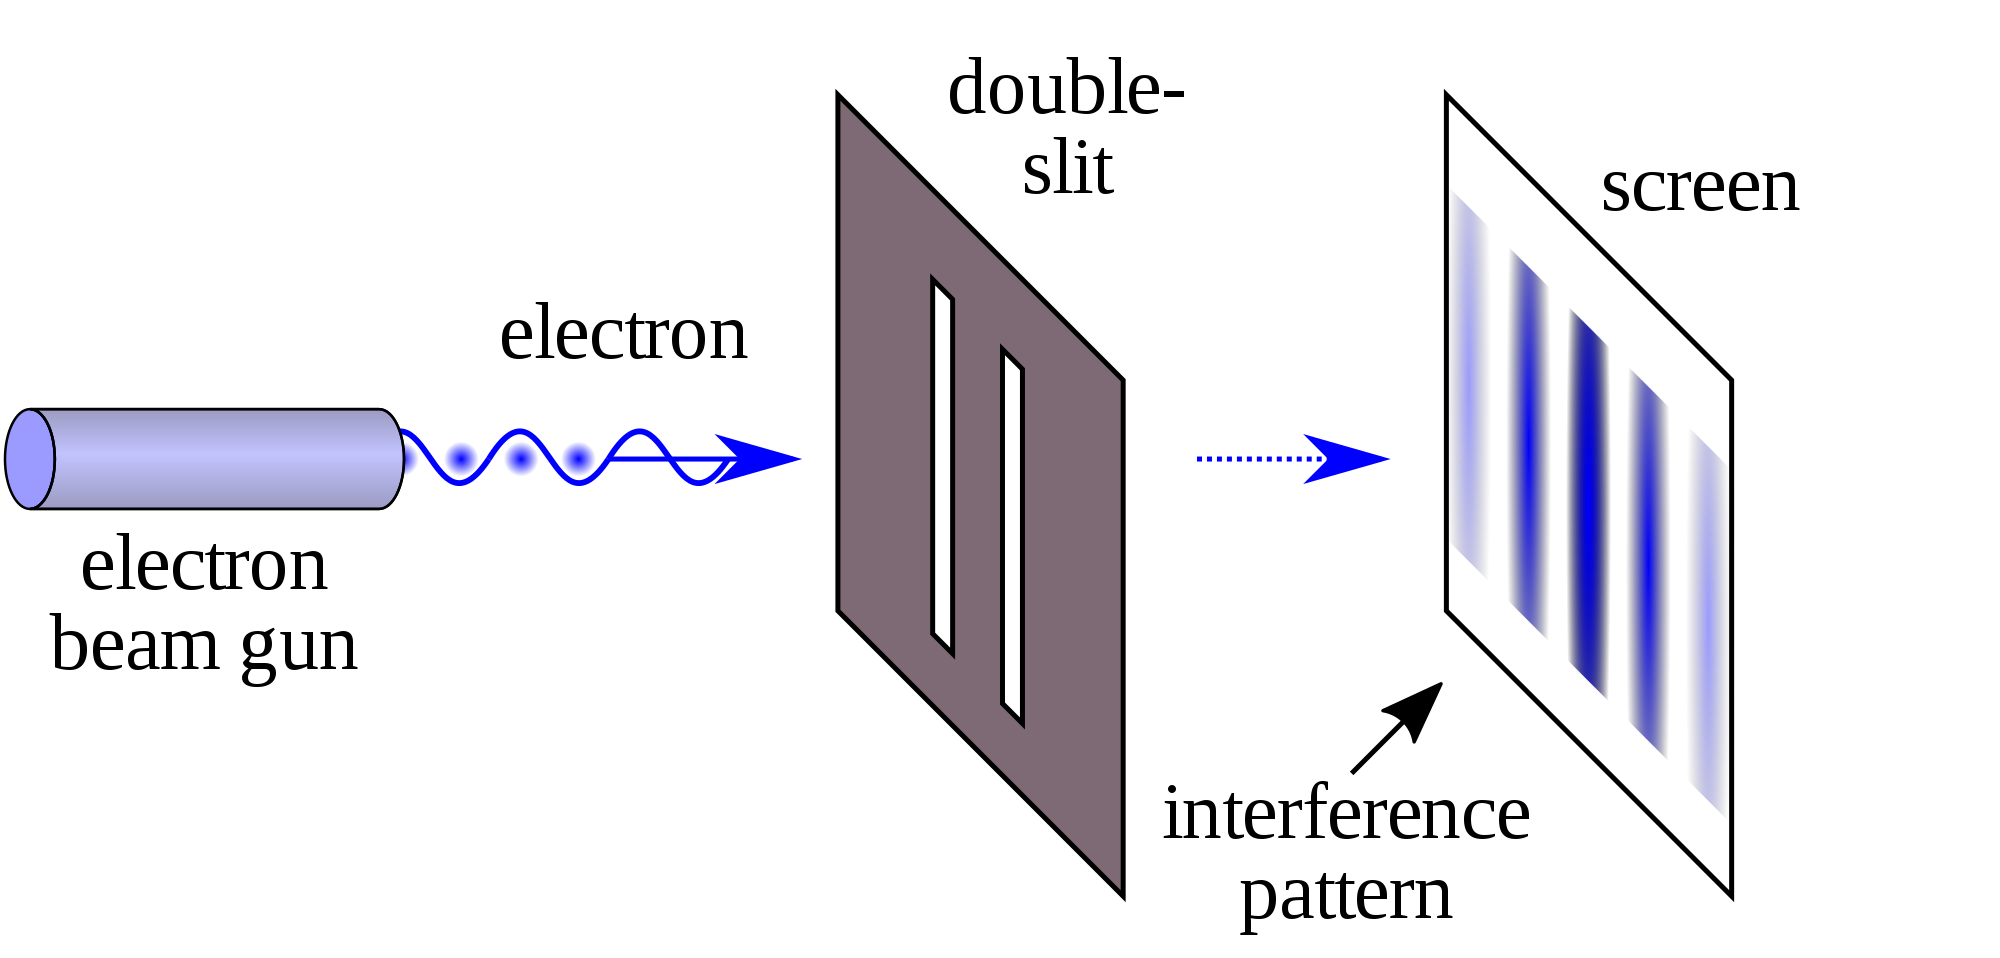
\includegraphics[width=0.6\textwidth]{figs/Etwoslitexp.png} \\
        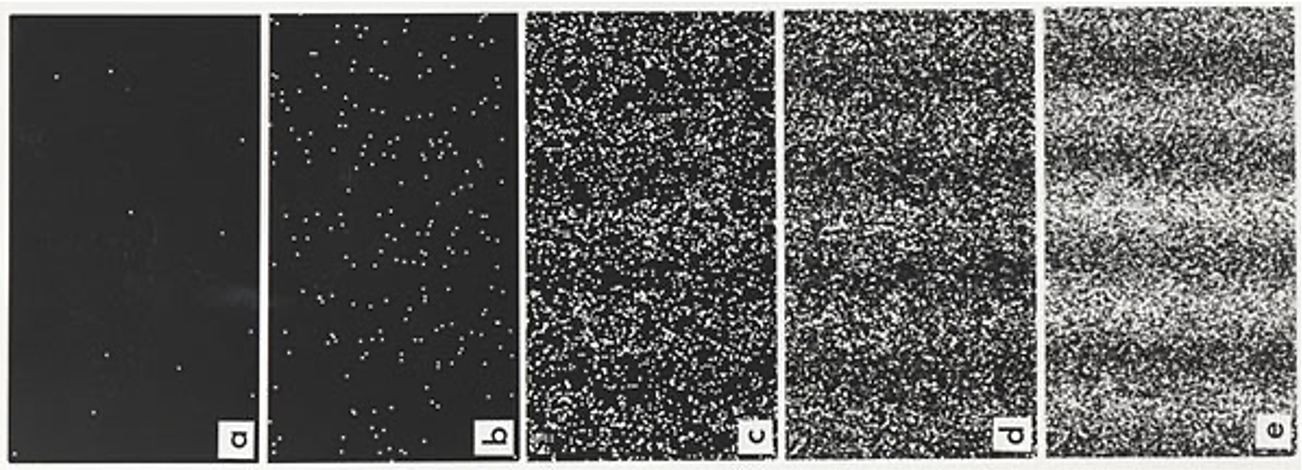
\includegraphics[width=0.6\textwidth]{figs/two-slit.png} \\
    \end{center} 
\end{frame}

\begin{frame}
    \frametitle{}
    实验分析:\\
    \begin{itemize}
        \Item 多个波构成电子 
        \Item 多个电子构成 
        \Item 单个电子既是粒子又是波 
    \end{itemize}
\end{frame}

\begin{frame}
    如果单个电子既是粒子又是波 \\
\begin{itemize}
    \Item  电子与自己干涉 
    \Item  电子同时过两个缝  
    \Item  电子至少同时有两条路径 
    \Item  牛顿力学失效! 
    \Item  波动学失效! 
\end{itemize}
\end{frame}

\begin{frame}
    \centering
    \begin{tcbb}[0.68]{波粒二象性导致的困境}
        {如何描述象电子这样具有波粒二象性物体的运动?}
    \end{tcbb}
\end{frame}

%%%%%%%%%%%%%%%%%%%%%
\subsection{波函数假说}
%%%%%%%%%%%%%%%%%%%%%

\begin{frame}
    \frametitle{波函数假说}
    \begin{tcolorbox4}[Basic assumption 1/5]
    In 1924, De Broglie assumed that:\\
    ~\\
    The state of matter is described by a wavefunction \\
    ~\\
    (物体的状态用波函数描述)
    \end{tcolorbox4}
\end{frame}

\begin{frame}
    \frametitle{}
    构造第一个波函数(平面波函数):~\\
    For the classical plane wave,
        \begin{equation*}
            \begin{split}
                y(x,t)&=A e^{i(\frac{2\pi}{\lambda}x-\omega t)} \\
                    & = A e^{i\frac{2\pi}{h}(\frac{h}{\lambda}x-h\nu t)}
            \end{split} 
        \end{equation*}
        Put De Broglie relationship into the formula, we get a quantum plane wavefunction
        \begin{equation*}
            \begin{split}
                \Psi_p(x,t)&=A e^{\frac{i}{\hbar}(px-Et)}
            \end{split} 
         \end{equation*}
         It describes the state of a quantum free particle\\
         \Note ~ A wavefunction is a complex function 
\end{frame}

\begin{frame}
         For a general wavefunction, it should be a wave-packet of plane wavefunction
         \begin{equation*}
                \Psi(x,t)=\sum\limits_{p} c(p)\Psi_p(x,t) = \int\limits_{-\infty} ^{\infty} c(p,t) e^{\frac{i}{\hbar}px}dp
         \end{equation*}
\end{frame}


\begin{frame}
    \frametitle{德布罗意}
        \begin{columns}
            \begin{column}[t]{0.46\linewidth}
                主要成就:\\
                \begin{enumerate}
                    \Item 物质波假说
                    \Item 原子内电子的波动性
                    \Item 波函数假说 
                    \Item 构造第一个波函数
                \end{enumerate}
                ~\\
                \begin{quote}
                "德布罗意已经揭开了面纱的一角"  \\
                    \rightline{$\cdots$ 爱因斯坦 (1925)\hspace{3em}}
                \end{quote}  
            \end{column}
            \begin{column}[t]{0.46\linewidth}
                \begin{center}
                    \includegraphics[width=0.85\textwidth]{figs/2021-12-03-18-00-05.png} \\
                \end{center} 
            \end{column}
        \end{columns}
\end{frame}

%%%%%%%%%%%%%%%%%%%%%%%%%%%%%%%%%
\section{2.波函数统计诠释}
%%%%%%%%%%%%%%%%%%%%%%%%%%%%%%%%%

\subsection{统计诠释}
\begin{frame}
    \frametitle{统计诠释}
    In 1926, Born proposed statistical interpretation of wavefunction
    \begin{tcolorbox4}[Statistical interpretation]
        \large The magnitude of wavefunction $\Psi(\vec{r},t)$ does not tell us how much of 
        the particle is at position $\vec{r}$ at time t, 
        but rather the probability (W) that the particle is at or near the position at time t. \\
        \[ d W = |\Psi(\vec{r},t)|^2 d \tau \]
    \end{tcolorbox4}
    {\color{deepred} Nobel Prize in physics(1954)}
\end{frame}

\begin{frame}
    \frametitle{}
    解释干涉实验:
    \begin{itemize}
        \Item 自由电子是平面波,可等概率出现在屏的任一位置
        \Item 电子波通过双缝发生衍射和干涉,导致某些位置的振幅大,某些位置的振幅小
        \Item 振幅较大的位置电子出现的概率大,形成明纹。振幅小的位置电子出现的概率小,形成暗纹
        \Item 明暗干涉条纹不体现电子波的形状,体现的是电子出现概率的分布
    \end{itemize}  
\end{frame}

\subsection{统计诠释的数学描述}

\begin{frame}[allowframebreaks=]
    统计诠释的数学描述:
    \begin{enumerate}
        \Item Probability density \[\omega = |\Psi|^2 =\Psi^* \Psi \]
        \Item Probability  \[ d W = |\Psi|^2 d \tau \]
        \Item Normalization \[ \int_{\Omega} |\Psi|^2 d \tau =1 \]
        \Item Momentum wavefunction \[ c(\vec{p},t)=\frac{1}{(2\pi\hbar)^{3/2}} \int_{-\infty}^{\infty} \Psi(\vec{r},t) e^{\frac{-i}{\hbar} \vec{p}\cdot \vec{r} } d \tau \] 
        \Item Expectation value of any function $f (x)$  \[ <f(x)>=\int_{-\infty}^{\infty} f(x) |\Psi(x)|^2 dx \]
        \Item Expectation value of observable A \[ <A>=\int_{-\infty}^{\infty} \Psi^*(x) [A \Psi](x)| dx \]
    \end{enumerate}
\end{frame}

\begin{frame}
    \frametitle{}
    \Tips \\
    \begin{itemize}
        \Item $\Psi$ and $C\Psi$ describe the same state 
        \[ \frac{C\Psi(x_1)}{C\Psi(x_2)} = \frac{\Psi(x_1)}{\Psi(x_2)}\]
        \Item $\Psi$ and $e^{i\varphi}\Psi$ describe the same state 
         \[ |e^{i\varphi}\Psi|^2 = e^{-i\varphi} e^{i\varphi} |\Psi|^2 = |\Psi|^2 \] 
    \end{itemize}  
    * 两相同的波叠加, 在测量上并没有什么不同,与经典条件下两相同的波叠加完全不同
\end{frame}

\begin{frame}
    Statistical interpretation requires wavefunctions to be (标准化条件):
    \begin{itemize}
        \Item finite  function
        \Item continuous function 
        \Item monotropic function
        \Item square integrable function 
    \end{itemize}
\end{frame}

\begin{frame}[allowframebreaks=]
    \frametitle{}
    \EXP[1.~normalizating the wavefunction] {\[\psi(x)=\sin(x), \qquad (0\le x \le \pi)\]}
    \Solution ~assuming the normalized wavefunction to be 
    $\Psi=C\sin(x)$
    \begin{equation*}
        \begin{split}
            \int_0 ^\pi |C\sin(x)|^2 dx &=1 \\
            C^2 \int_0 ^\pi \sin^2(x) dx &=1 \\
            C^2 \int_0 ^\pi \frac{1-\cos 2x }{2} dx &=1 \\ 
            C^2 [\frac{x}{2}-\frac{\sin 2x}{4}]_0 ^\pi &=1 \\ 
        \end{split} 
     \end{equation*}
     \[C=\sqrt{\frac{2}{\pi}}\]
     The normalized wavefunction:
     \begin{equation*}
        \Psi=C\sin(x)=\sqrt{\frac{2}{\pi}}\sin(x)
    \end{equation*}
\end{frame}

\begin{frame}[allowframebreaks=]  
    \EXP[2.~normalizating the plane wavefunction ] {\[\Psi_p (x,t)=e^{\frac{i}{\hbar}(px-Et)} \] }
    \Solution  ~assuming the normalized wavefunction 
    $\Psi=C\Psi_p (x,t)$
    \begin{equation*}
        \begin{split}
            \int_{-\infty} ^\infty |C\Psi_p (x,t)|^2 dx &=1  \\
            C^2 \int_{-\infty} ^\infty \Psi_p (x) \Psi_{p} ^* (x) dx &=1  \\
            C^2 \int_{-\infty} ^\infty \Psi_p (x) \Psi_{p'} ^* (x) dx &=\delta (p-p')  \\
            C^2 \int_{-\infty} ^\infty e^{\frac{i}{\hbar}(p-p')x} dx &=\delta (p-p')\\
        \end{split} 
     \end{equation*}
     with the defination of $\delta$ funcation,
     \[ \delta(x)=\int_{-\infty}^{+\infty} \frac{d k}{2 \pi} e^{i k x}\]
     we get
     \[C^2 2\pi \hbar \delta (p-p') =\delta(p-p') \]
     \[C= \dfrac{1}{\sqrt{2\pi \hbar}}\]
     The normalized plan wavefunction:
     \begin{equation*}
        \Psi=\frac{1}{\sqrt{2\pi \hbar}} e^{\frac{i}{\hbar}px}
    \end{equation*}  
    In general
    \[ \Psi(\vec r ,t)=\frac{1}{(2\pi \hbar)^{3/2}} e^{\frac{i}{\hbar}(\vec p\cdot \vec r -Et)} \]
    \[ \Psi(\vec r_1 ,\vec r_2, t)=\frac{1}{(2\pi \hbar)^{6/2}} e^{\frac{i}{\hbar}(\vec p_1 \cdot \vec r_1 +\vec p_2 \cdot \vec r_2 -Et)} \]
\end{frame}

\begin{frame}
    \frametitle{玻恩 (Max Born)}
        \begin{columns}
            \begin{column}[t]{0.46\linewidth}
                主要成就:
                \begin{enumerate}
                    \Item 波函数的统计诠释
                    \Item 态叠加原理
                \end{enumerate}
                德国理论物理学家,量子力学的奠基人之一。\\
                因对波函数的统计解释,获1954年诺贝尔物理学奖.\\
                1912年受聘哥廷根大学无薪讲师,1933年因犹太血统被剥夺教职和财产,流亡英国.\\ \vspace{0.3em}
                泡利、海森堡和黄昆都是他的学生
            \end{column}
            \begin{column}[t]{0.46\linewidth}
                \begin{center}
                    \includegraphics[width=0.9\textwidth]{figs/Born.png} \\
                \end{center} 
            \end{column}           
        \end{columns}
\end{frame}

\begin{frame}  
    \begin{tcolorbox3}[Conclusion]
        ~~\\
       {The state of matter is described by a wavefunction and the magnitude of the wavefunction $ \Psi(x,t)$ 
       tells us the probability that the particle is at or near the position ($x$) at time $t$.}
    \end{tcolorbox3} 
\end{frame} 

\begin{frame}
    \frametitle{}
    \centering
    \tcbb[0.5]{Big problems}
    {
    {Is the world obeys the rule of probability ?}
    }
\end{frame}
 %%%%%%%%%%%%%%%%%%%%%%%%%%%%%%%%%%%%%%%%%%%%%%%%%%%%%%%%%%%%%%%%%%%
 \begin{frame}
     \frametitle{课外作业}
     \begin{enumerate}
        \item 已知氢原子电子的波函数(t=0)为$\psi(r)=Ae^{-r/a_0} $,试求:\\
               (1) 归一化系数A \\
               (2) 电子在$r-r+dr$之间出现的概率\\
               (3) 电子在哪里出现概率最大(r的值) 
        \item 已知氢原子电子的波函数(t=0)为$ Y_{10} $,试求:\\
                (1) 电子在$(\theta, \varphi) -(\theta + d \theta, \varphi + d \varphi)$之间出现的概率\\
                (2) 电子在哪个方位出现的概率最大 
     \end{enumerate}
 \end{frame}
 %%%%%%%%%%%%%%%%%%%%%%%%%%%%%%%%%%%%%%%%%%%%%%%%%%%%%%%%%%%%%%%%%%%

 \section{3.态叠加原理}

 \begin{frame}
     \frametitle{前情回顾}
     \begin{itemize}
         \Item 波粒二象性
         \Item 波函数假说
         \Item 波函数统计诠释
     \end{itemize}
 \end{frame}  
 
 \subsection{态叠加原理实验基础}
 
 \begin{frame}
     \frametitle{两种双缝实验}
         \begin{figure}
             \centering
             \subfigure[小球双缝实验]{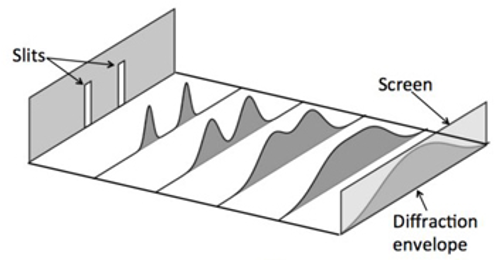
\includegraphics[width=0.49\textwidth]{figs/2022-01-17-13-50-38.png}}
             \subfigure[电子双缝实验]{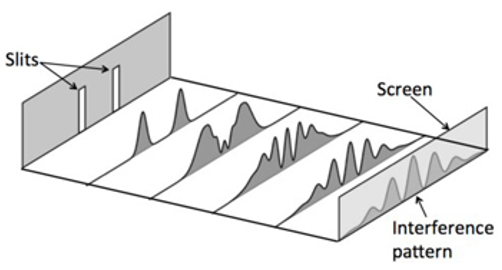
\includegraphics[width=0.49\textwidth]{figs/2022-01-17-13-51-15.png}}
         \end{figure}
     \setcounter{subfigure}{0}
 \end{frame}
 
 \begin{frame}
     \frametitle{小球双缝实验}
     \begin{center}
         \includegraphics[width=0.5\textwidth]{figs/sup-2.png} \\
     \end{center} 
     依据统计诠释,振幅是概率幅\\
     \begin{itemize}
         \Item 小球双缝实验,$P'=P_1+P_2 $, 是概率叠加。
         \Item 结论:经典叠加服从概率叠加
     \end{itemize}
 \end{frame} 
 
 
 \begin{frame}
     \frametitle{电子双缝实验}
     \begin{center}
         \includegraphics[width=0.5\textwidth]{figs/sup-3.png} \\
     \end{center} 
     依据统计诠释,振幅是概率幅\\
     \begin{itemize}
         \Item 电子双缝实验,$P\neq P_1+P_2 $,量子叠加服从的不是概率叠加!
         \Item 波恩认为服从波函数(态)叠加,即:
         $$ \psi =\psi_1+\psi_2$$
     \end{itemize}
 \end{frame} 
 
 
 \begin{frame} [allowframebreaks=]
     \tikzstyle{na} = [baseline=-.5ex]
     Analysing the two-slit experiment:\\
     \begin{itemize}
         \Item Using wavefunction $\psi_1$ to describe the state of the electron running across slit-1 and $\psi_2$ for slit-2. \\
         \Item when the both slits opened, one can assume that the electron locates at the superposition state
             \[ \Psi=c_1 \psi_1+ c_2\psi_2 \]
         \Item based on statistical interpretation, the possiblity density of electron reaches certain point of screen should be
         \begin{equation*}
         \begin{split}
             \omega &=|\Psi|^2 \\
             &= (c_1 \psi_1+ c_2\psi_2)^* (c_1 \psi_1+ c_2\psi_2) \\
             &=(\psi_1^*+\psi_2^*)(\psi_1+\psi_2) \\ 
             & = |c_1|^2 |\psi_1|^2 + |c_2|^2 |\psi_2|^2  
             + \Myitem{t1}{red}{[c_1 c_2 ^* \psi_1 \psi_2 ^* + c_1 ^* c_2 \psi_1 ^* \psi_2]} \\
         \end{split} 
         \end{equation*}
     \end{itemize}
     \begin{itemize}
         \Item 概率计算表明,电子处于叠加态时,存在干涉项(后两项),产生干涉条纹
         \Item 如果电子不处于叠加态,即电子只过一个缝,则有$\psi_1$ 或$\psi_2$为零,不存在干涉项,没有干涉条纹!
         \Item 干涉条纹正是源于电子同时过两个缝的状态, 即叠加态。
     \end{itemize}
     基于此,波恩提出了态叠加原理
 \end{frame}
 
 \subsection{态叠加原理表述}
 
 \begin{frame}
     \frametitle{态叠加原理}
     Born also proposed that: \\
     \begin{tcolorbox4}[Superposition principle of states]
     If $\psi_1$ and $\psi_2$ are the possible states of the system,
     their linear superposition \[ \Psi=c_1 \psi_1+ c_2\psi_2 \]
     is also the possible state of the system.\\
     if the system locates at the superposition $\Psi$, the possiblity of observating the system at $\psi_1$ is $|c_1|^2$, and at $\psi_2$ is $|c_2|^2$ \\
     \[|c_1 |^2 + |c_2 |^2 =1\]
     \end{tcolorbox4}
 \end{frame}
 
 \begin{frame}
     \frametitle{}
     \begin{tcolorbox4}[态叠加原理中文表述]
     如果 $\psi_1$ 、 $\psi_2$、 $\cdots$、$\psi_N$ 是粒子可能的态,那么它们的线性叠加
         $$ \Psi=c_1 \psi_1+ c_2\psi_2+\cdots+c_N\psi_N $$
     也是粒子可能的态(叠加态)\\   
     如果粒子处于叠加态 $\Psi=\sum\limits_{i=1}^N c_i \psi_i$,  
     那么测得粒子处在第$i$态 ($\psi_i$) 的概率为 $|c_i |^2$, 
     并且有  $$\sum_{i=1}^{N} |c_i|^2 =1$$
     \end{tcolorbox4}
     ~~\\ 
     * 经典叠加物体并不部分地处于原来各波的状态,测量时也得到原来各波的值!
 \end{frame}
 
 \subsection{波函数坍塌}
 
 \begin{frame}
     \frametitle{实验升级}
     \begin{center}
         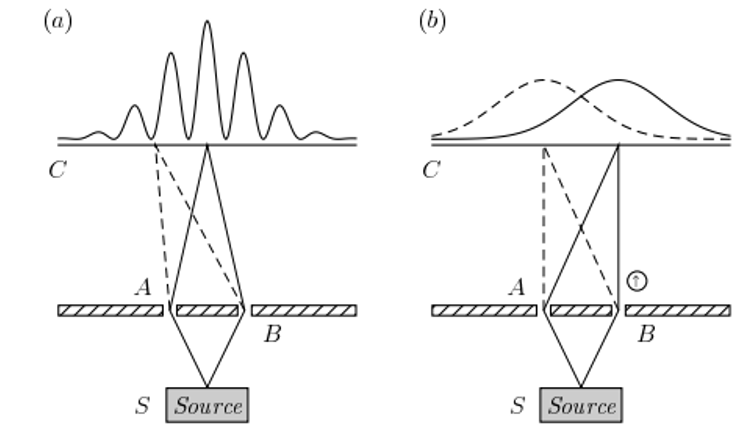
\includegraphics[width=0.5\textwidth]{figs/sup-4.png} \\
     \end{center} 
     \begin{itemize}
         \Item 目标:观测电子是如何同时过两条缝的
         \Item 结果:1)只能测到电子要么过第一缝,要么过第二缝。\\
         2)探测器越灵敏,干涉条纹越模糊,\\
         3)当探测器能长时间地保持几乎可以完全判断电子过哪条缝时,干涉条纹消失!如图(b)所示
     \end{itemize}
 \end{frame}
 
 \begin{frame} 
     \frametitle{结果分析}
     \begin{enumerate}
         \Item 实验目标与实验结果的一致性\\
         \begin{itemize}
             \IItem 当我们“挖出”A和B两条狭缝时,“设计”了一个想要观察“波动性”的设备,也就是电子已经预先被我们设定为“波”,因此观测到波动性(干涉条纹)
             \IItem 当我们装上侦测器时,整个实验被我们“设计”成观察“粒子性”,因为想要知道电子到底是由A还是B穿过,就必须先具备确定的“位置”,因此观察到粒子性(干涉条纹消失)
         \end{itemize}
         \Item 测量可导致状态改变\\
         \begin{itemize}
             \IItem 探测前,电子处于叠加态($ \psi =\psi_1+\psi_2$)
             \IItem 探测时,电子状态改变,被迫从叠加态变为确定态 ($\psi_1$ or $\psi_2$),(称为波函数坍塌)
             \IItem 探测后,电子处于某确定态,不能干涉。
             \IItem 探测器不灵敏,有部分没有被探测到的电子处于叠加态, 干涉条纹模糊。
             \IItem 探测器灵敏,全部电子被探测,没有电子处于叠加态, 干涉条纹消失。
         \end{itemize}
     \end{enumerate}
 \end{frame}
 
 \begin{frame}   
     \begin{enumerate}
         \Item 测量结果的互补性(互补性原理)\\
         \begin{itemize}
             \IItem 波动性和粒子性是两种不同的属性,一般不能用同一设备进行测量
             \IItem 不能因为测得粒子性就否定波动性,反之亦然。
             \IItem 测量结果就算相互矛盾,也要同时接受,因为它们互补地揭示物体的本质。
         \end{itemize}
         \Item 结论
         \begin{itemize}
             \IItem 电子具有波粒二象性,总是处于叠加态
             \IItem 不被测量,则保持在叠加态
             \IItem 测量导致确定态,但结果是随机的。
             \IItem 测得电子过某条缝,不能说明电子原本就要过这条缝,为只是测量导致的结果
         \end{itemize}
     \end{enumerate}
 \end{frame}
 
 \subsection{学术大讨论}
 \begin{frame}
     \frametitle{学术大讨论}
     The probabilistic interpretation was controversial from the beginning of of quantum mechanics
     \begin{tcolorbox4}[Which Way?]
     \begin{itemize}
         \Item De Broglie : Pilot waves
         \Item Schr$\ddot{o}$dinger: Schr$\ddot{o}$dinger's cat
         \Item Einstein: EPR paradox
         \Item Wheeler's delayed choice experiment
         \Item Quantum eraser experiment
         \Item $\cdots \cdots$
     \end{itemize}
     \end{tcolorbox4}
 \end{frame}
 
 \begin{frame}
     \frametitle{薛定谔的猫}
     \begin{center}
         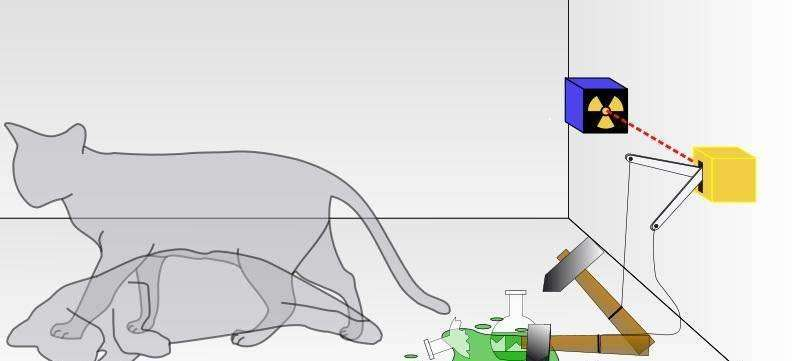
\includegraphics[width=0.9\textwidth]{figs/2022-03-04-13-49-09.png} \\
     \end{center} 
 \end{frame}
 
 \begin{frame}
     \frametitle{EPR佯谬}
     \begin{center}
         \includegraphics[width=0.9\textwidth]{figs/28.png} \\
     \end{center} 
 \end{frame}
 
 \begin{frame}
     \frametitle{贝尔不等式}
     \begin{center}
         \includegraphics[width=0.8\textwidth]{figs/bell.png} \\
     \end{center} 
 \end{frame}
 
 \begin{frame}
     \frametitle{惠勒延迟选择实验}
     \begin{center}
         \includegraphics[width=0.7\textwidth]{figs/choose.png} \\
     \end{center} 
 \end{frame}
 
 \begin{frame}
     \frametitle{量子擦除实验}
     \begin{center}
         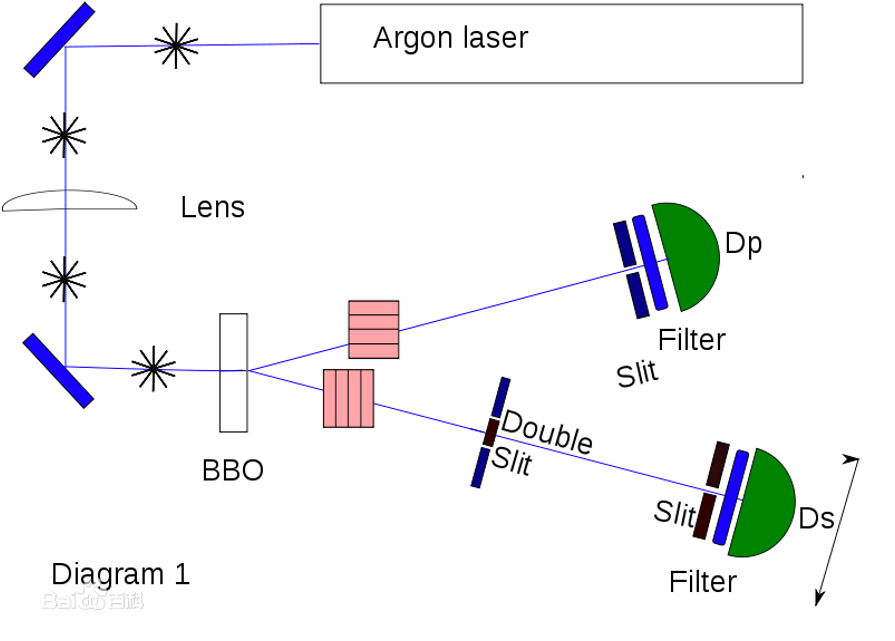
\includegraphics[width=0.7\textwidth]{figs/c1.png} \\
     \end{center} 
 \end{frame}
 
 \begin{frame}
     \frametitle{}
     \begin{center}
         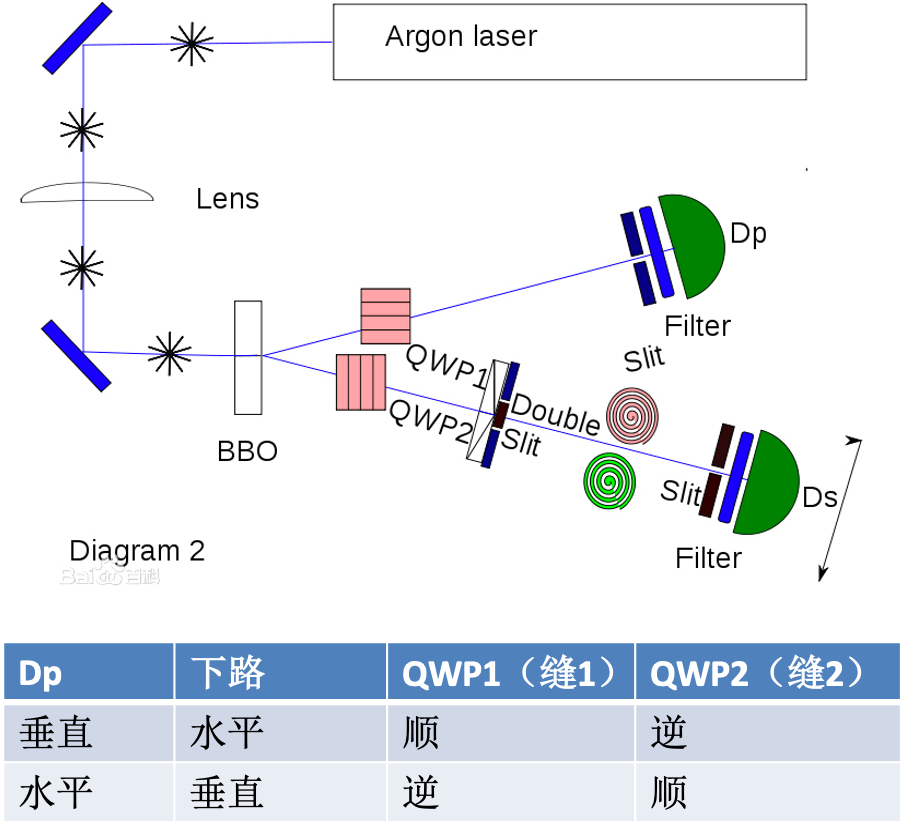
\includegraphics[width=0.6\textwidth]{figs/c2.png} \\
     \end{center} 
 \end{frame}
 
 \begin{frame}
     \frametitle{}
     \begin{center}
         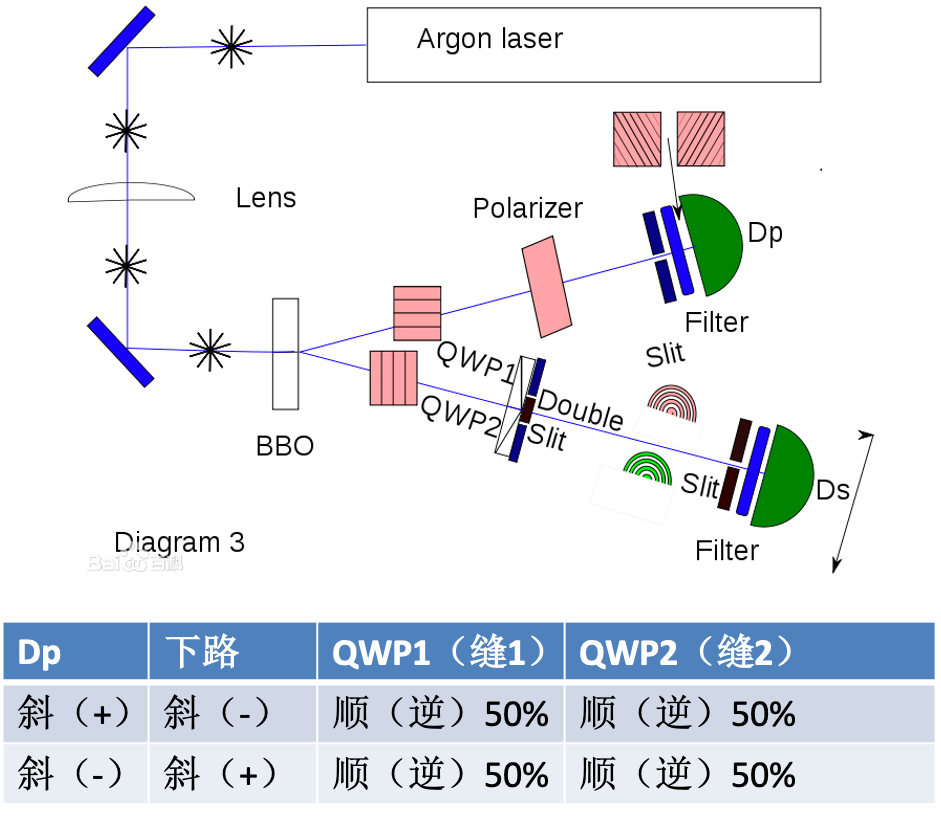
\includegraphics[width=0.6\textwidth]{figs/c3.png} \\
     \end{center} 
 \end{frame}
 
 \begin{frame}
     \begin{tcolorbox4}[Conclusion]
         ~~\\
     \begin{enumerate}
         \Item Objects are wave-particles and in superposition state
         \Item Measurement changes the state and gives random results
         \Item Measurement results are complementary
         \Item Measurement leads to objective reality
     \end{enumerate}
     \end{tcolorbox4}
 \end{frame}
 
 \begin{frame}
     \frametitle{}
     \centering
     \tcbb[0.5]{Big problems}
     {
       \large  {The world is not a real world?\\
       What is the measurement? \\
       If not performing measurement, what it should be?}
     }
 \end{frame}
 
  %%%%%%%%%%%%%%%%%%%%%%%%%%%%%%%%%%%%%%%%%%%%%%%%%%%%%%%%%%%%%%%%%%%
  \begin{frame}
     \frametitle{课外作业}
     \begin{enumerate}
        \item 已知粒子的波函数(t=0)如下,
            \[\psi(x) = \begin{cases}
              \sqrt{A}\sin \frac{\pi x}{a}, \quad 0\leq x\leq a\\
              0, \qquad  x<0, x>a
            \end{cases}\]
                (1)试求归一化系数A \\
                (2)试求位置的概率密度 \\
                (3)试求动量的概率密度
        \item 试用态叠加原理解释电子双缝干涉实验
     \end{enumerate}
 \end{frame}
 %%%%%%%%%%%%%%%%%%%%%%%%%%%%%%%%%%%%%%%%%%%%%%%%%%%%%%%%%%%%%%%%%%%
 

\section{4.薛定谔方程}

\begin{frame}
    \frametitle{前情回顾}
    \begin{itemize}
        \Item 波粒二象性
        \Item 波函数假说
        \Item 波函数统计诠释
        \Item 态叠加原理
    \end{itemize}
\end{frame}  

\begin{frame}
    \begin{tcolorbox4}[Conclusion]
        ~~\\
    \begin{enumerate}
        \Item Objects are wave-particles and in superposition state
        \Item Measurement changes the state and gives random results
        \Item Measurement results are complementary
        \Item Measurement leads to objective reality
    \end{enumerate}
    \end{tcolorbox4}
\end{frame}  

\begin{frame}
    \centering
    \tcbb[0.5]{Big problems}
    {
      If not performing measurement, what it would be? 
    }
\end{frame}

\subsection{波函数演化假说}

\begin{frame}
    \begin{tcolorbox4}[Basic assumption 2/5]
        The evolution of wavefunction obeys Schr$\ddot{o}$dinger equation
        \begin{equation*}
            i\hbar \frac{\partial }{\partial t} \Psi (\overrightarrow{r},t ) =\left [ -\frac{\hbar^2}{2\mu }\nabla ^2 + V(\overrightarrow{r},t ) \right ]\Psi (\overrightarrow{r}, t ) 
        \end{equation*}
    \end{tcolorbox4}
\end{frame}

\subsection{薛定谔方程}

\begin{frame}
    \frametitle{神秘来源}
    \begin{itemize}
        \Item 1923年,德布罗意博士论文传到了瑞士,一战炮兵指挥官苏黎世大学讲师薛定谔作了一个关于物质波假说的报告,德拜评注:\\
        $$\text{“有了波,总得有个波动方程吧”}$$
        \Item 1926年,薛定谔:
        $$“Dear~Debye, I~find~one~\cdots”$$
    \end{itemize}            
\end{frame}

\begin{frame}
    \begin{alertblock} {}  
    \begin{quote}
        “是粒子还是波?是妻子还是情人?这都是难题!” \\
        ~~\\
        \rightline{--《薛定谔的女友》(2001)\hspace{6em}}   
    \end{quote}  
    \begin{quote}    
    这部话剧讲述了薛定谔方程建立的神秘过程:在1925年圣诞节前,薛定谔像往年一样,来到阿尔卑斯山度假。这次陪伴他的不是妻子安妮,而是维也纳的一位神秘女郎。
    就是这位比薛定谔的猫还神秘的女郎激发了薛定谔的灵感,使他在一年的时间里连发~6~篇~“SCI”~论文,建立波动量子力学,$\cdots$\\
    ~~\\
    \end{quote} 
    \end{alertblock}   
\end{frame}

\begin{frame}
	\begin{alertblock} {可能思路}  
		\begin{itemize}
			\Item 	\textbf{1:}  最小作用量原理 $\int\limits_{t_1}^{t_2} \delta L d t =0 $\\ 
			\Item 	\textbf{2:}  波粒二象性\\ 
			~\\ 
			\Item 	\textbf{3:}  基本假设,不能从现有理论推导\\
            ~\\ 
            \begin{quote}
            "It is not possible to derive it from anything you know. It came out of the \alert{\faHeartbeat} of Schr$\ddot{o}$dinger"\\
            \rightline{$\cdots$ R. P. Feynman \hspace{3em}}   
            \end{quote}
		\end{itemize}
	\end{alertblock}
\end{frame}

\begin{frame} [allowframebreaks=]
    \frametitle{}
    \alert{\faHeartbeat} Quantum plane wavefunction \[\psi(x,t)=\Psi_p(x,t)=e^{\frac{i}{\hbar}(p\cdot x-Et)} \]
    should be a sulotion of this equation
    \begin{equation*}
        \begin{split}
       -i\hbar \nabla \psi(x,t) &=p\psi(x,t) \\ \vspace{0.6em}
       \hbar^2 \nabla^2 \psi(x,t) &=p^2\psi(x,t) \\
       \frac{\hbar^2}{2\mu} \nabla^2 \psi(x,t) &=\frac{p^2}{2\mu} \psi(x,t) , \qquad \cdots (1)
        \end{split}
    \end{equation*}
    \begin{equation*}
       i\hbar \frac{\partial }{\partial t} \psi(x,t) =E\psi(x,t)  , \qquad \cdots (2)
     \end{equation*}
    (2)-(1)
    \begin{equation*}
        (i\hbar \frac{\partial }{\partial t} - \frac{\hbar^2}{2\mu} \nabla^2 )\psi(x,t) =(E-\frac{p^2}{2\mu})\psi(x,t)=0  
    \end{equation*}
    \begin{equation*}
        i\hbar \frac{\partial }{\partial t} \psi(x,t) = \frac{\hbar^2}{2\mu} \nabla^2 \psi(x,t)
    \end{equation*}
    For general wavefunction, it's a wave packet of plane wavefunction
    \begin{equation*}
        \Psi(x,t)= \int\limits_{-\infty} ^{\infty} c(p,t) e^{\frac{i}{\hbar}px}dp
    \end{equation*}
    we get 
    \begin{equation*}
        \begin{split}
        (i\hbar \frac{\partial }{\partial t} - \frac{\hbar^2}{2\mu} \nabla^2 )\Psi(x,t) &= \int\limits_{-\infty} ^{\infty} c(p,t) (E-\frac{p^2}{2\mu}) e^{\frac{i}{\hbar}px}dp=0  \\
        i\hbar \frac{\partial }{\partial t} \Psi(x,t) &= \frac{\hbar^2}{2\mu} \nabla^2 \Psi(x,t)
        \end{split}
    \end{equation*}
    For nonfree particle in a potential $U(x)$,
    \begin{equation*}
        \boxed{i\hbar \frac{\partial }{\partial t} \Psi(x,t) = (\frac{\hbar^2}{2\mu} \nabla^2 +U(x)) \Psi(x,t)}
    \end{equation*}
    That is the Schr$\ddot{o}$dinger equation. \\
    ~~\\
    {\Bullet} For N-particles system
   {\small \begin{equation*}
        i\hbar \frac{\partial }{\partial t} \Psi(x_1, x_2, \cdots x_N,t) = [\sum_{i=1} ^{N} \frac{\hbar ^2}{2\mu_i} \nabla^2 +U(x_1, x_2, \cdots x_N)] \Psi(x_1, x_2, \cdots x_N,t)
    \end{equation*}}
\end{frame}

\begin{frame}
    \frametitle{}
    检验正确性:
    \begin{enumerate}
        \Item 自由粒子的解 ~~ 求解自由粒子的一维薛定谔方程
        \Item 氢原子光谱
        \Item $\cdots \cdots$
    \end{enumerate}
    ~\\ 
    发表论文:《Quantisierung als Eigenwert problem》(量子化是本征值问题),整整140页!
\end{frame}

\begin{frame}{名人评述}
    \begin{enumerate}
        \Item 
        \begin{quote}
            “我一阅读完毕整篇论文,就像被一个迷语困惑多时渴慕知道答案的孩童,现在终于听到了解答!” \\
            ~~\\
            \rightline{--普朗克(1926)\hspace{5em}}   
        \end{quote}  
        \Item 
        \begin{quote}
            “这著作的灵感如同泉水般源自一位真正的天才!” \\
            ~~\\
            \rightline{--爱因斯坦(1926)\hspace{4em}}   
        \end{quote}  
        \Item  
        \begin{quote}
            “你的方程把量子理论推进了关键性的一步!” \\
            ~~\\
            \rightline{--玻尔(1926)\hspace{6em}}   
        \end{quote} 
    \end{enumerate}
\end{frame}

\begin{frame}
    \frametitle{薛定谔}
    \begin{wrapfigure} {r} {0.3\textwidth} %;图在右
        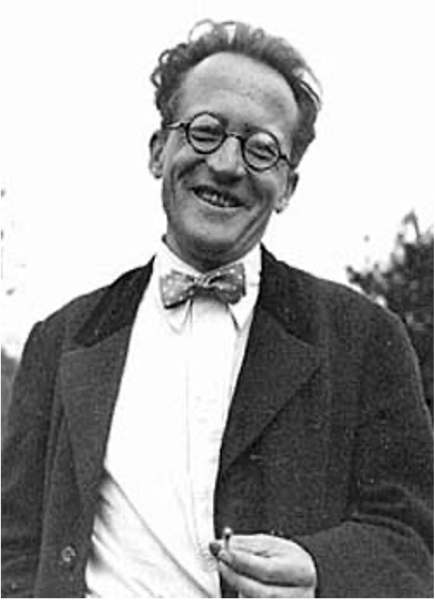
\includegraphics[width=0.25\textwidth]{figs/schroginger.png}   
    \end{wrapfigure}
奥地利理论物理学家, 生于维也纳, 量子力学的奠基人之一。薛天才,通灵的人, 1926年提出薛定谔方程,获1933年诺贝尔物理学奖; 1935年提出“薛定谔的猫”,至今还是“养猫人”的猫王;1943年写的《生命是什么》一书,被誉为“唤起生物革命的小册子”。\\ \vspace{0.3em}
薛定谔:他玉树临风,英俊潇洒,风流倜傥,人见人爱,花见花开,情人无数,江湖人称“段正淳"
\end{frame}

\begin{frame}
    \frametitle{}
    \centering
    \tcbb[0.68]{Significance }
    {
      \large {It's the most fundamental equation in quantum mechanics. 
      It's the starting point for every quantum mechanical system we want to describe: electrons, protons, neutrons, whatever.
      And now, it has become the established analogue of Newton's second law of motion for quantum mechanics}
    }
\end{frame}

\subsection{守恒定律}

\begin{frame} 
    \frametitle{守恒定律 }
    {\Bullet} 概率守恒定律\\ \vspace{0.3em}
    守恒定律关心的是物理量随时间的变化率问题,量子力学中最重要的是概率,我们考虑概率密度的变化率
    $$\omega (\vec{r}, t)=|\Psi(\vec{r}, t)|^{2}=\Psi^{*}(\vec{r}, t) \Psi(\vec{r}, t)$$
    \begin{equation*}
        \begin{split}
            \frac{\partial \omega}{\partial t} &=\Psi^{*} \frac{\partial \Psi}{\partial t}+\frac{\partial \Psi^{*}}{\partial t} \Psi, \cdots (1) \\
            \frac{\partial \Psi}{\partial t} & =\frac{i \hbar}{2 \mu} \nabla^{2} \Psi+\frac{1}{i \hbar} U \Psi, \cdots (2) \\
            \frac{\partial \Psi^{*}}{\partial t} & =-\frac{i \hbar}{2 \mu} \nabla^{2} \Psi^{*}-\frac{1}{i \hbar} U \Psi^{*}, \cdots (3) 
        \end{split}
    \end{equation*}
\end{frame}

\begin{frame} 
    把(2)(3)代回(1),得:
    \begin{equation*}
        \begin{split}
        \frac{\partial \omega}{\partial t}
        &=\frac{i \hbar}{2 \mu}\left(\Psi^{*} \nabla^{2} \Psi-\Psi \nabla^{2} \Psi^{*}\right) \\
        &=\frac{i \hbar}{2 \mu}[(\Psi^{*} \nabla^{2} \Psi + \nabla \Psi^{*} \nabla \Psi)- (\nabla \Psi^{*} \nabla \Psi +\Psi \nabla^{2} \Psi^{*})] \\ 
        &=\frac{i \hbar}{2 \mu} \nabla \cdot\left(\Psi^{*} \nabla \Psi-\Psi \nabla \Psi^{*}\right)\\
        &=-\nabla \cdot \frac{i \hbar}{2 \mu} \left(\Psi \nabla \Psi^{*}-\Psi^{*} \nabla \Psi\right) \\
        &=-\nabla \cdot \vec{J}
        \end{split}
    \end{equation*}
\end{frame}

\begin{frame} 
    上式定义了一个矢量: $\vec{J}=\dfrac{i \hbar}{2 \mu} \left(\Psi \nabla \Psi^{*}-\Psi^{*} \nabla \Psi\right) $,  得连续性方程(4),\\
    \begin{equation*}
        \frac{\partial \omega}{\partial t}+ \nabla \cdot \vec{J}=0, \cdots (4)
    \end{equation*}    
    说明矢量 $\vec{J}$ 的散度决定了概率密度变化率。\\ \vspace{0.6em}
    在任意空间区域 V, 对(4)式求积分,有:
    \begin{equation*}
        \frac{d}{d t} \int_{V} \omega d \tau =-\int_{S} \vec{J} \cdot d \vec{S}, \cdots (5)
    \end{equation*}
    由 Gauss 定理可知,单位时间内体系V内增加的概率应等于穿过V边界面S进入V内的概率,所以$\vec{J}$是概率流。(4) 式和(5)分别是概率守恒定律的微分和积分形式。\\ \vspace{0.3em}
\end{frame}

\begin{frame} \frametitle{}   
    {\Bullet} 粒子数守恒定律\\ \vspace{0.3em}
    \begin{equation*}
        \begin{split}
        \frac{d}{d t} \int\limits_{V\to\infty} \omega d \tau &= \frac{d}{d t} \int\limits_{V\to\infty} |\Psi(\vec{r}, t)|^{2} d \tau  \\
        &=\frac{d}{d t} 1\\ 
        &=0
        \end{split}
    \end{equation*}
    说明全空间概率不随时间发生变化,即粒子既未产生也未湮灭时,概率守恒定律就是粒子数守恒定律。\\ \vspace{0.3em}
\end{frame}

\begin{frame}\frametitle{}
    {\Bullet} 质量守恒定律\\ \vspace{0.3em}
    对(4)式,左右两边同乘以粒子的质量$\mu$, 
    \begin{equation*}
        \frac{\partial \mu\omega}{\partial t}+ \nabla \cdot \mu\vec{J}=0
    \end{equation*}  
    得质量守恒定律
    \begin{equation*}
        \frac{\partial \omega_\mu}{\partial t}+ \nabla \cdot \vec{J_\mu}=0, \cdots (6)
    \end{equation*} 
\end{frame}

\begin{frame}\frametitle{}
    {\Bullet} 电荷守恒定律\\ \vspace{0.3em}
    对(4)式,左右两边同乘以粒子的电荷$e$, 
    \begin{equation*}
        \frac{\partial e\omega}{\partial t}+ \nabla \cdot e\vec{J}=0
    \end{equation*}  
    得电荷守恒定律
    \begin{equation*}
        \frac{\partial \omega_e}{\partial t}+ \nabla \cdot \vec{J_e}=0, \cdots (7)
    \end{equation*}  
\end{frame}

\subsection{定态薛定谔方程}

\begin{frame} 
    \frametitle{定态问题}
    若势函数$V(\vec{r},t ) $不显含时间 t,则时间变量可分离 \\ \vspace{0.3cm}
    方程: { $ \displaystyle i \hbar \frac{\partial }{\partial t} \Psi (\vec{r},t ) =\left [- \frac{\hbar^2}{2\mu }\nabla ^2 + V(\vec{r}) \right ]\Psi (\vec{r},t ) $}  \\  \vspace{0.3cm}
    \alert{解:}  设  $\Psi (\vec{r},t )  = \Psi (\vec{r} ) f(t) $ , 代回方程 \\ 
     { $ \displaystyle i\hbar \Psi (\vec{r})  \frac{\partial }{\partial t} f(t)=f(t) \left [ -\frac{\hbar^2}{2\mu }\nabla ^2 + V(\vec{r}) \right ]\Psi (\vec{r}) $}  \\ 	
     { $ \displaystyle i\hbar \frac{1}{f(t)}  \frac{\partial }{\partial t} f(t)= \frac{1}{\Psi (\vec{r}) } \left [ -\frac{\hbar^2}{2\mu }\nabla ^2 + V(\vec{r}) \right ]\Psi (\vec{r}) =E $}  \\ \vspace{0.3cm} 
     得两个微分方程:\\  \vspace{0.3cm}
     I、演化方程  $ \displaystyle  i\hbar \frac{1}{f(t)}  \frac{\partial }{\partial t} f(t)=E, \qquad $  
        解方程,得:$\displaystyle  f(t) =e^{-iEt/\hbar}$ 
\end{frame}

\begin{frame} 
    II、定态薛定谔方程 $\displaystyle   \left [ -\frac{\hbar^2}{2\mu }\nabla ^2 + V(\vec{r}) \right ]\Psi (\vec{r}) =E \Psi (\vec{r})  $   \\ 
    算符形式:$$\displaystyle   \hat{H} \Psi (\vec{r}) =E \Psi (\vec{r})  $$   
    是哈密顿算符 $\hat{H}$ 的本征方程。结合定解条件,可得能量本征值($E_n$)及本征函数 $\Psi_{E_n} (\vec{r} )$ \\ \vspace{0.6em}
    \begin{definition}[定态:]
        \hspace{2em}能量有确定值的态称为定态,用定态波函数描述
        \[ \Psi_{E_n} (\vec{r} ) e^{-i E_n t/\hbar} \] 
    \end{definition}
    依据态叠加原理,一般的态(叠加解)可表示为:
    \[ \Psi (\vec{r},t ) =\sum\limits_n c_n(t)\Psi_{E_n} (\vec{r} ) e^{-iE_n t/\hbar}  \]
\end{frame}

\begin{frame} 
    \frametitle{定态的概率与概率流}
    \例[1.试证明定态的概率密度不随时间变化]{}
    \证~
    \begin{equation*}
        \begin{split}
            \omega (\vec{r}, t)&=\Psi^{*}(\vec{r}, t) \Psi(\vec{r}, t) \\
            &=\Psi_{E_n} (\vec{r} ) e^{-iE_n t/\hbar} \Psi_{E_n} ^* (\vec{r} ) e^{iE_n t/\hbar} \\
            &=\Psi_{E_n} (\vec{r} )\Psi_{E_n} ^* (\vec{r} ) \\
            &=|\Psi_{E_n} (\vec{r} )|^2
        \end{split}
    \end{equation*}
\end{frame}

\begin{frame}   
    \例[2.试证明定态的概率流密度不随时间变化]{} 
    \证~ 
    \begin{equation*}
        \frac{\partial \omega}{\partial t }+ \nabla \cdot \vec{J}=0
    \end{equation*}  
    \to
    \begin{equation*}
        \nabla \cdot \vec{J}=-\frac{\partial \omega}{\partial t}=0
    \end{equation*}  
\end{frame}

\begin{frame}
    \frametitle{学术讨论}
    问题:体系总是处于叠加态,不测量时,波函数服从薛定谔方程演化,测量时波函数坍塌(Collapsing waves),导致客观实在。那坍塌过程服从什么规律?\\
    \begin{center}
        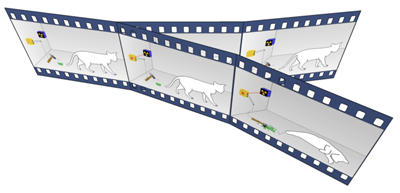
\includegraphics[width=0.6\textwidth]{figs/2022-01-17-13-13-18.png} \\
    \end{center} 
    \begin{quote}
    "Anyone who claims to understand quantum theory is either lying or crazy." \\
    \rightline{$\cdots$ R. P. Feynman \hspace{3em}}   
    \end{quote}
\end{frame}

%%%%%%%%%%%%%%%%%%%%%%%%%%%%%%%%%%%%%%%%%%%%%%%%%%%%%%%%%%%%%%%%%%%
\begin{frame}
    \frametitle{课外作业}
    \begin{enumerate}
        \item 已知粒子的波函数为$\psi(x,t)=Ae^{\frac{i}{\hbar}(p_x x - E t)}$,试求:\\
                (1)归一化系数A\\
                (2)概率密度$\omega(x,t)$\\
                (3)概率流密度$\vec{J}(x,t)$
        \item 如果势场$U(x,t)$不显含$x$,试求解一维薛定谔方程. 
        \item 设电子处于如下球型无限深势阱
        \[ U(r)= \begin{cases}
            0, \quad r<r_0
            \infty \quad r\geq r_0
        \end{cases} 
        \]
        试求电子的能级及径向波函数$\psi(r)$
    \end{enumerate}
\end{frame}
%%%%%%%%%%%%%%%%%%%%%%%%%%%%%%%%%%%%%%%%%%%%%%%%%%%%%%%%%%%%%%%%%%%

